% \documentclass{report}
\documentclass[11pt]{article}
\setlength{\columnsep}{0.8cm}
\usepackage{fullpage}
\usepackage[english]{babel}
\usepackage{blindtext}
\usepackage{amssymb}
\usepackage{graphicx}
\usepackage{wrapfig}
\usepackage{tabularx}
\usepackage{multirow}
\usepackage{amsmath}
\usepackage{mathtools}
\usepackage{graphicx}
\usepackage{caption}
\usepackage{subcaption}

% \usepackage{algorithm}
% \usepackage{algorithmic}
\usepackage{algorithmicx}
\usepackage{algpseudocode}
% \pagenumbering{gobble}

% \setlength{\parindent}{0pt}
% \setlength{\intextsep}{0cm}

\author{6.867 Homework 2 and 3}
\begin{document}
\noindent\centerline{\LARGE{Two-Variable Recommendation Models}}
\noindent\centerline{}
\noindent\centerline{}
\noindent\centerline{Fall 2014}
\noindent\centerline{6.867 Final Project}
\noindent\centerline{Geoffrey Gunow and Neha Patki}

\section{Introduction}
In 2014, Yelp published an academic dataset containing over 42,000 businesses that span 5 metropolitan areas. Types of data included the full star rating, and reviews for each business, as well as aggregated statistics for each user's reviews. In this project, we use the dataset to formulate, model, and solve the problem of estimating a user's overall review for a business, given the user's history. The algorithm we present estimates a single rating, but can be applied to multiple business to determine the best one for a given user. Thus, our problem falls in the category of recommendation systems.

\subsection{Motivation}
Yelp does not currently give personal recommendations to its users, but the data it collects about reviews and users make it possible to learn a user's preferences. Typical approaches fall in two categories. Collaborative filtering analyzes similarities between different users, and the items they rate highly. Content-based filtering focuses on a single user's personal history to determine individual likes and dislikes.

For Yelp's data set, we find that a collaborative filter would not take into account an individual's own preferences for cuisines and restaurant sub-categories. However, we cannot use pure content-based filtering because a single user may not have reviewed a significant number of restaurants, making the data points sparse. This motivates us to use a hybrid approach in estimation, where we combine a user's history with a cluster-based approach meant to account for the sparsity of data points. We introduce a hidden variable that models an overall group of similar users, and use this variable to separately learn preferences for each group.

An additional challenge and motivation for the problem is analyzing the given data to determine relevant features. Yelp offers a vast array of data ranging from the ambiance in each restaurant, to the number of times a user was voted funny by their peers. Furthermore, the 5 metropolitan areas are diverse in their offerings of food, and users may show preferences towards particular types of restaurants. We spend a significant time engineering feature vectors to reflect the variety of information. After the learning process, this enables us to comment on significant features to reveal trends in user preferences. 

\subsection{Problem Formulation}
The overall goal is to accept, as inputs, a user and business, and to output a floating point value in $[1, 5]$ that predicts what the user will rate the business. We do this using two steps.

\begin{enumerate}
\item Categorize the users into groups who have roughly similar interests. This is the hidden variable.
\item Separetely train each category to learn the average business rating for only the users in that group.
\end{enumerate}

For example, assume a particular group we learn in step 1 contains users who prefer Mexican restaurants. In step 2, the expected output is the average rating given only by its members. This means that another group may be trained to rate the same business differently, which shows its users have different broad preferences. Figure \ref{fig:system} shows an overall schematic of the system.\\

\begin{figure}[h!]
    \centering
    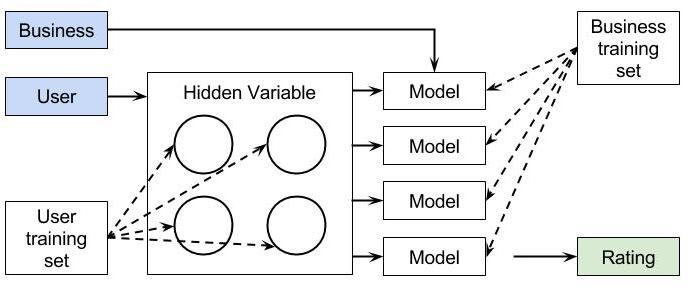
\includegraphics[width=0.9\textwidth, height=6cm]{system}
    \caption{The architecture for the overall system. Inputs are colored blue while the output is shown in green. Dotted lines represents inputs during training, and solid lines represent the flow of information at testing time. The hidden variable is used to select a model, or a mixture of models, that the business data is tested on. The output is the rating.}
    \label{fig:system}
\end{figure} 

Modeling the hidden variable in step 1 is an unsupervised learning problem, because we are constructing groups for which we have no prior labels. However, after learning the hidden variable, the step 2 is fully supervised because we are presented with a full list of ratings for each business. Considering the full system, we see that we can perform an end-to-end test given a user, a business, and an expected rating. This allows us to indirectly supervise the hidden variable to determine the appropriate hyperparameters for step 1. The overall complexity of our system grows, and we perform a train-validate-test strategy recursively for step 2 within the context of the overall system.

In the next sections, we discuss constructing the feature vectors that create the user and business data shown in Figure \ref{fig:system}. We describe multiple approaches to implement both variables, and describe our train-validate-testing strategy. Finally, we compare the different methodologies in terms of accuracy.

\section{Features}

A key to success in any machine learning problem is the selection of relevant features to accurately represent the data of interest. While algorithms are important, the success that can be achieved is often bounded by the ability of the features to accurately represent the problem. In our project, we need to develop two sets of features. The first set of features corresponds to user attributes that will be used to predict the hidden class associated with each user. The second set corresponds to business attributes that will be used to predict how a user in a given class will rate a business.

\subsection{User Data}
The Yelp dataset is comprised of three relevant files: a user review file, a user attribute file, and a business attribute file. A straightforward approach would be to classify a user based purely off the data presented in the user attribute file. This file contains information about the user along with a user ID. However, the information provided is only basic with attributes such as the total number of reviews a user has written, the average of the user's ratings, and less relevant attributes such the user's full name.

Therefore, we use a different approach to form user features. We still take a couple features from the user attribute file, namely the user's average rating and the total number of reviews, but most features are formed by cross referencing the user's ID with the user reviews file. With our approach, we find the reviews associated with the user's ID and store the rating and business ID associated with each review. Then from the business ID we can cross reference the business file to determine the type of business.  Yelp lists categories associated with each business. For instance, every restaurant will have the string `restaurant' in its categories but might also have the string `Mexican restaurant.'

This allows us to form features that describe how a user prefers different types of businesses. In particular, there is a feature associated with the user's average rating for businesses in each category along with another feature for the frequency a user has reviewed each category. To compensate for users that preferentially give good or bad reviews, the user's average rating is subtracted from the category-averaged rating. Therefore these features provide information on the user's preferences in businesses, such as liking Italian food but disliking Mexican food.

One major challenge with this approach is missing data. For the vast majority of users, there will be categories in which the user has given no reviews. For most machine learning algorithms, the data needs to be complete. To remedy this, we choose to fill missing data using data imputation. We assign the user's average review to categories in which the user has no reviews. Since we subtract by the user's average review in category ratings, this corresponds to inserting zeros for these missing features. 

Typically, data imputation is not the appropriate method to solve the missing data problem for large data sets \cite{em_vs_im}. The preferred method is expectation-maximization (EM) in which the objective function is directly maximized \cite{em}. However, EM presents a few problems for our scheme. Fist, there is a large amount of missing data. For almost all users there is more than one missing feature value. In addition, many clustering algorithms do not work well with the probabilistic approach of EM. In EM, no single value is assigned to missing data points. Instead, a probability is assigned. In an iterative process estimates for this probability are updated along with density estimation parameters. Some clustering algorithms such as k-means do not perform density estimation but rather partition the feature space \cite{kmeans}. This is problematic since EM requires evaluation of the likelihood of the data.

Overall, the user feature vector contains 33 features, 28 of which are associated with the average rating and number of reviews for 14 categories of businesses. The remaining 5 features are statistical features associated with the user, such as variance of review ratings and average review rating. The only difference between the restaurant and nightlife problems is that the categories are different. All of the features for restaurant categories are presented in Table~\ref{tab:user_features1} with features for nightlife categories presented in Table~\ref{tab:user_features2}. Statistical features, which take the same form in both problems, are presented in Table~\ref{tab:user_features3}

Similarly, for nightlife businesses the user feature vector contains 32 features. The only difference is that the business categories are slightly different. These are 

\begin{table}[h!]
	\caption{User Feature Descriptions (Restaurant Categories)}
	\centering
	\begin{tabular}{c|c|c}
		Restaurant Category & \multicolumn{2}{c}{Feature Numbers} \\ \hline
		& Review Frequency & Scaled Review Average \\
		Mexican & 0 & 14 \\
		American (Traditional) & 1 & 15\\
		Fast Food & 2 & 16\\
		Pizza & 3 & 17\\
		Sandwiches & 4 & 18\\
		Nightlife & 5 & 19\\
		Bars & 6 & 20\\
		Food & 7 & 21\\
		American (New) & 8 & 22\\
		Italian & 9 & 23\\
		Chinese & 10 & 24\\
		Burgers & 11 & 25\\
		Breakfast/Brunch & 12 & 26\\
		Japanese & 13 & 27\\
	\end{tabular}
	\label{tab:user_features1}
\end{table}

\begin{table}[h!]
	\caption{User Feature Descriptions (Nightlife Categories)}
	\centering
	\begin{tabular}{c|c|c}
		Nightlife Category & \multicolumn{2}{c}{Feature Numbers} \\ \hline
		& Review Frequency & Scaled Review Average \\
		Wine Bars & 0 & 14 \\
		Jazz Clubs & 1 & 15\\
		Gay Bars & 2 & 16\\
		American (Traditional) & 3 & 17\\
		Breweries & 4 & 18\\
		Karaoke & 5 & 19\\
		Dive Bars & 6 & 20\\
		Restaurants & 7 & 21\\
		Bars & 8 & 22\\
		Lounges & 9 & 23\\
		Dance Clubs & 10 & 24\\
		Sports Bars & 11 & 25\\
		Pubs & 12 & 26\\
		Music Venues & 13 & 27\\
	\end{tabular}
	\label{tab:user_features2}
\end{table}

\begin{table}[h!]
	\caption{User Feature Descriptions (Statistics)}
	\centering
	\begin{tabular}{c|c}
		Feature & Feature Number \\ \hline
		Number of present user reviews & 28 \\
		Variance of present user ratings & 29 \\
		Average of present user ratings & 30 \\
		Total number of user reviews & 31 \\
		Average of total user ratings & 32 \\
	\end{tabular}
	\label{tab:user_features3}
\end{table}

\subsection{Business Data}

Once users are partitioned into clusters, a model must be developed for each cluster that predicts the business rating. To accomplish this, features related to the businesses are required. For this set, most features are pulled directly from the list of binary attributes. The business attributes are primarily binary features such as whether a restaurant allows smoking. However, again missing data is common in the business features.

For business features, missing data is treated differently than it was for user features. This is because missing business data directly corresponds to missing data in the Yelp dataset and might actually be representative of the business. For instance if the business is new or not very popular, many attributes corresponding to the business may be missing. For established businesses, we expect that more attributes will be present. 

Therefore, missing binary features are treated as categorical features. More specifically, we split each binary feature into three features. Only one feature is 1 and the other two are 0. If there is a present and positive binary feature, the first feature is marked with a 1. If there is a present and negative binary feature, the second feature is marked with a 1. In the case of missing data, the last feature in the set is marked with a 1. 

A similar approach is taken with actual categorical features. For instance, the attire attribute may be listed as casual, dressy, formal, or the data might be missing. This feature is therefore split into four features with an approach similar to the binary features wherein only one feature is marked with a 1.

Additional features are engineered from the data available. The Yelp dataset is based off data from 5 metro areas: Phoenix, Las Vegas, Madison, Waterloo, and Edinburgh. The business attributes lists the city in which the restaurant is located, but not the metro area. This is problematic since intuitively the metro area should have an impact on the rating since the five cities are very different in nature. However, the latitude and longitude of the locations is provided. Using these coordinates along with the coordinates of the centers of the major cities, as provided by Wikipedia, the metro area can easily be determined by finding the closest center. Therefore a categorical feature can be developed for the metro area much like the attire example presented previously. Additionally, distance to the center of the city might be important so a feature is added that gives the distance to the center of the city based off the coordinates.

\section{Methodology}
After constructing the feature vectors, our data now consists of a set $B$ of business vectors, and a set $U$ of user vectors. Assume the vectors are constructed as described in the previous section. We also have access a set of ratings, $R$, where a single rating is determined by a user and a business. Let $r_{ub} \in R$ denote the rating given by user $u$ to business $b$.

We first train the user vectors, $U$ with the hidden variable. This will return multiple sets of users, $U_s \subseteq U$.  We then define a function that takes in a set of users and a business, and outputs the average rating given to the business only by the users in the set. Mathematically, this is:

\begin{equation}
\label{basic}
f(U_s, b) = \frac{\sum\limits_{u \in U_i} r_{ub}}{|U_i|}
\end{equation}

Where $U_i \subseteq U_s$ is the set of users who have given a rating to business $b$. If $U_i = \emptyset$, then this function is not defined. 

We can then perform an inference method for the non-hidden variable.  We define its inputs and outputs in terms of the business vectors, $B$. As inputs, we have the set of businesses that some user in the set has rated. If the set is $U_s$, we denote the relevant set of businesses as $B_s$, where for every $b \in B_s$, $r_{ub}$ exists for at least one $u \in U_s$. Then the inference is trained with input $B_s$ and expected output $\{f(U_s, b)\}$, $\forall b \in B_s$.

We now present the three separate ways we formulated the problem to discover the sets of users, $U_s$. We also describe the methods of inference we use for the second variable.

\subsection{K-Means Clustering}
Perhaps the most naive way to calculate the hidden variable is to perform k-means clustering analysis using the set $U$ of training user vectors, and to use the cluster as the hidden variable. The different clusters are then trained separately. If we let $k$ be the number of clusters, then the k-means clustering will return sets of users $U_0, U_1, \ldots, U_{k-1}$ such that a user only belongs to one of the sets ($U_i \cap U_j = \emptyset$ for any $U_i \neq U_j$). Each of the clusters can then be trained independently using any method of inference.

It is important to note that for two different clusters of users, the businesses the users have rated are not necessarily identical. That is, for $U_i, U_j$ where $U_i \neq U_j$, it is not necessarily the case that $B_i = B_j$. Furthermore, if there does exist a $b \in B_i$ and $b \in B_j$, then it is not necessarily the case that $f(U_i, b) = f(U_j, b)$. This means that the same business vectors can be trained with different expected output based on the clusters. It represents our belief that the users in different clusters have different preferences, so they may rate the same business differently. 

Then, we can predict the rating given a user $u$ and a business $b$ by first finding its cluster, and then running the result of the inference method on the business vector.\\

\begin{algorithmic}[1]
\Function{predict}{$u, b$}
\State $i \gets$ cluster$(u)$ \Comment{A cluster number.}
\State method $\gets$ inference(cluster$=i)$ \Comment{The trained inference predictor for the cluster.}
\State \Return method$(b)$
\EndFunction
\end{algorithmic}
\medskip

Note that the complexity of this grows with the number of clusters we choose. With k clusters, finding the cluster in line 2 and the appropriate cluster's trained inference method in line 3 take $O(k)$ time.

\subsection{K-Neighbors}
A different approach determines the hidden clusters dynamically at run time. In this approach, we do not hard-code any clusters but decide them based on the input variables when testing. We perform a nearest-neighbors analysis, and let that particular set of users be the cluster used to perform the inference. Let $k$ be an integer that represents the number of neighbors we will use. Then at testing time, we find the $k$ nearest neighbors and perform an inference on these neighbors dynamically.\\

\begin{algorithmic}[1]
	\Function{predict}{$u, b$}
	\State $U_s \gets$ kNeighbors$(u)$, $Y \gets \small[ \small]$
	\State $B_i \gets$ businesses$(U_s)$ \Comment{Businesses users in $U_s$ have rated.}
	\For {$b \in B_i$}
	\State $r = f(U_s, b)$ \Comment{Returns average rating within $U_s$.}
	\State $Y \gets Y + r$
	\EndFor
	\State inference = train(input $=B_i$, output $=Y)$ \Comment{Prediction method.}
	\State \Return inference$(b)$
	\EndFunction
\end{algorithmic}
\medskip

Here, $U_s$ is the set of k nearest neighbors to $u$. In step 8, we train to learn the ratings that only users in set $U_s$ have given. This enables us to find the most similar users to the queried user, $u$, in real-time to dynamically train a model fitted to the user. Similar to the k-means algorithm, every set $U_s$ of users may be trained to learn the business ratings differently. Even though this method requires almost no work during training, it becomes expensive at test time because it is necessary to perform inference.

Note that the total number of unique sets $U_s$ of size $k$ is $|U| \choose k$. In theory, we could complete an inference algorithm on each of these sets during testing time, but we found this to be infeasible with a growing size of $U$ and $k$. Furthermore, dynamically performing the inference allows the model to be more flexible in that we can add more users to $U$ at any point, or change the parameter $k$. The downside is that each prediction takes a longer time to run because there is a complete inference problem that must be solved for every queried $u, b$ pair. 

\subsection{Mixture of Gaussians}
Our third model treats clustering using a probabilistic approach. Assuming that the users in $U$ are a mixture of several Gaussian distributions allows us to treat a single user, $u$, as probabilistically belonging to different clusters. If we choose $k$ as the number of mixtures (our hyperparameter), this means that asking to cluster a user $u$ will return a list of size $k$, where each element $i$ is in $[0, 1]$. This represents the probability of user $u$ belonging to mixture $i$.

During training time we perform $k$ inference algorithms, one for each mixture, similar to the k-means method. However, instead of completely partitioning the users into clusters, we use all users and weight them based on how likely they are to belong there. Let $p_i(u)$ be the probability that user $u$ belongs to cluster $i$. Our calculation of the rating then takes a different form.

\begin{equation}
\label{weighted}
g(i, b) = \frac{\sum\limits_{u \in U} r_{ub}p_i(u)}{\sum\limits_{u \in U} p_i(u)}
\end{equation}

Here $i$ is the index assigned to a particular mixture. For each mixture, we consider all the users in $U$, but the ratings of these users are weighted according to how likely it is the user belongs to $i$. We can think of this as a more general form of Equation \eqref{basic}, which treats the weights as a continuous probability in $[0, 1]$ instead of a discrete value $\{0, 1\}$.

During testing time, we are given a user $u$ and can similarly calculate the probability that the user belongs to the different mixtures. We can use this to either choose the maximum likelihood estimate, or weight the different clusters to convey our uncertainty.


\subsubsection{Maximum Likelihood Estimate}
In the case of the maximum likelihood estimate, this strategy works similarly to k-means clustering. Though the underlying Gaussian mixture model is different, we perform the same analysis at testing time. Given a user $u$, we find the cluster, $i$, that has the maximum probability $p_i(u)$. We can then use a trained inference model for the $i^{th}$ cluster with a business, $b$, to compute our prediction of the rating.

\subsubsection{Probabilistic Weights}
In this case, we must perform the trained inference for each mixture and output the weighted result of all mixtures, according to the probabilities of the user belong to that mixture.\\

\begin{algorithmic}[1]
	\Function{predict}{$u, b$}
	\State $p \gets$ mixture$(u)$ \Comment{List of probabilities.}
	\State total $\gets 0$
	\For{$p_i \in p$} \Comment{Weight of mixture $i$.}
	\State method $\gets$ inference(cluster $=i)$ \Comment{Trained inference for mixture $i$.}
	\State total $\gets$ total + $p_i($method$(b))$
	\EndFor
	\State \Return $total$
	\EndFunction
\end{algorithmic}
\medskip

Similar to the k-means algorithm, this algorithm also grows linearly with the number of mixtures, $k$, because we enter the loop in line 4 exactly $k$ times. Note that the sum of all entries in $p$ must equal to 1, so it is not necessary to normalize the value stored in the $total$ variable.

\subsection{Inference Algorithms}
In each of the above cases, we have mentioned that after discovering an individual cluster, or mixture, we are able to perform an inference algorithm. Any inference algorithm we use must be able to accept, as inputs, a list of business features, $B$, along with the expected output $Y$, which are the corresponding ratings. It must output a function that is able to predict a rating, $r$ given a business vector $b$. This part can be directly supervised because we are provided with all the ratings each user has given to a business.

We consider 5 different algorithms when performing the inference.

\begin{itemize}
\item MLE: The maximum likelihood estimate just returns the average rating from all the given ratings. This is used as a benchmark for testing how the other algorithms compare.
\item Ridge: This is the ridge regression, as implemented in class.
\item Lasso: This is the lasso regression, as implemented in class.
\item Bayesian Ridge: This is a ridge-type regression that assumes all the input data is Bayesian. We were motivated to try this because we expected a user's ratings patterns to follow roughly a bell-shaped distribution.
\end{itemize}

For each of the three hidden-variable methods (K-Means, K-Neighbors, and Mixture of Gaussians), we test the inference algorithms above after we determine the appropriate cluster, or mixture of clusters.

\section{Experiments}
From the Yelp data set, we pulled out businesses that were categorized as `Restaurants' to narrow the scope. After doing so, we had a total of 14,304 business data points, and 12,596 user data points. The rest of this section describes our strategy for training, validating, and testing this data on the methods described previously. We then present our experimental results from running the data, both in terms of accuracy and time efficiency.

\subsection{Setup}
Our overall setup implemented a recursive train-validation-test strategy. Note that our method implements the overall problem of predicting a rating given a user, business pair. It does so in two steps:
\begin{enumerate}
\item Using the user as the input, determine the hidden variable. This is either a single cluster, or a mixture of clusters.
\item Using the cluster and the business as inputs, predict the overall rating.
\end{enumerate}

Step 2 can be directly supervised because we are given the actual average rating for a business. Thus, we can tune hyperparameters to the inference problem using the same train-validation-test strategy used in class by splitting the business data into 3 categories.

The problem is that step 1 cannot be supervised because it is a hidden variable, even though we need to tune its hyperparameters (the number of clusters, number of nearest neighbors, or number of mixtures). To solve this problem, we note that we can perform end-to-end testing on the entire system. Given a user and a business, we know what the overall rating should be. This means that we can split the user data into 3 categories as well, training the entire system, and validating the system end-to-end to determine the hyperpameters of the hidden variable. Figure \ref{fig:testing} shows a visual schematic of our testing system.

\begin{figure}[h!]
    \centering
    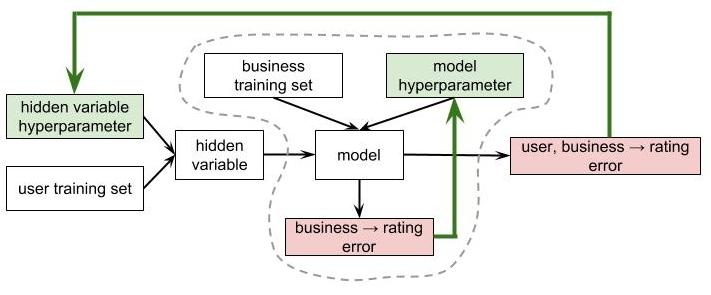
\includegraphics[width=0.9\textwidth, height=6cm]{testing_v2}
    \caption{The overall testing strategy shown for a single model. The model is trained to take in a business and compute the expected rating. As shown by the dashed line, it is a sub-problem within the overall system. When tested end-to-end, it outputs the expected rating for a user, business pair. Red boxes represent the two types of error that we can measure. The green arrows represent which hyperparameters the validation data is affecting.}
    \label{fig:testing}
\end{figure} 

The strategy works so that we recursively train-validate-test the business data for every model within a single iteration of training the user data. When we perform validation within the model, represented by the dashed gray area in Figure \ref{fig:testing}, we are testing predictions on businesses that the model has not seen before, but for the same users. In contrast, when we perform end-to-end testing, we are making predictions on users and businesses that the overall system has not seen. We chose a scheme where we used 50\% of the user data and business data to train, 25\% of the data to validate, and 25\% to test.

\subsection{Results}
We now present the results we achieved for each of the variables, as well as the overall end-to-end testing. While the hidden variable method was not supervised, we still present significant trends and comment on the perceived efficiency. In the overall system, we present validation accuracies for different hyperparameters.

\subsubsection{Hidden Variable}
The first step in our scheme is to cluster users based on the user feature vectors $U$. Included in this data is information about how often users have reviewed several categories of restaurants along with their rating for each category relative to their average rating. Additional features include the total number of reviews. 
 
If we use this raw data in a K-Means clustering algorithm, we observe very poor results. This is due to some features having much greater values and deviation, therefore receiving more weight. In particular, the total number of businesses a user has reviewed can have a large value whereas the average rating of a category relative to the user average is real valued in the range (0,4). This leads to average category ratings having little impact on the clustering. To avoid this, each feature is scaled relative to the mean and standard deviation of that feature in the dataset \cite{kmeans}. For every feature $\phi^d_i$ corresponding to the $d^{\text{th}}$ feature for user $i$, the scaled feature value $\tilde{\phi^d_i}$ is calculated as
 \begin{equation}
\tilde{\phi^d_i} = \frac{\phi^d_i - \mu^d}{\sigma^d}
 \end{equation}
 where $\mu^d$ is the average value for feature $\phi^d$ in the dataset with standard deviation $\sigma^d$. This limits the effect a single feature can have on influencing the cluster boundaries.
 
 \begin{figure}[h!]
 	\centering
 	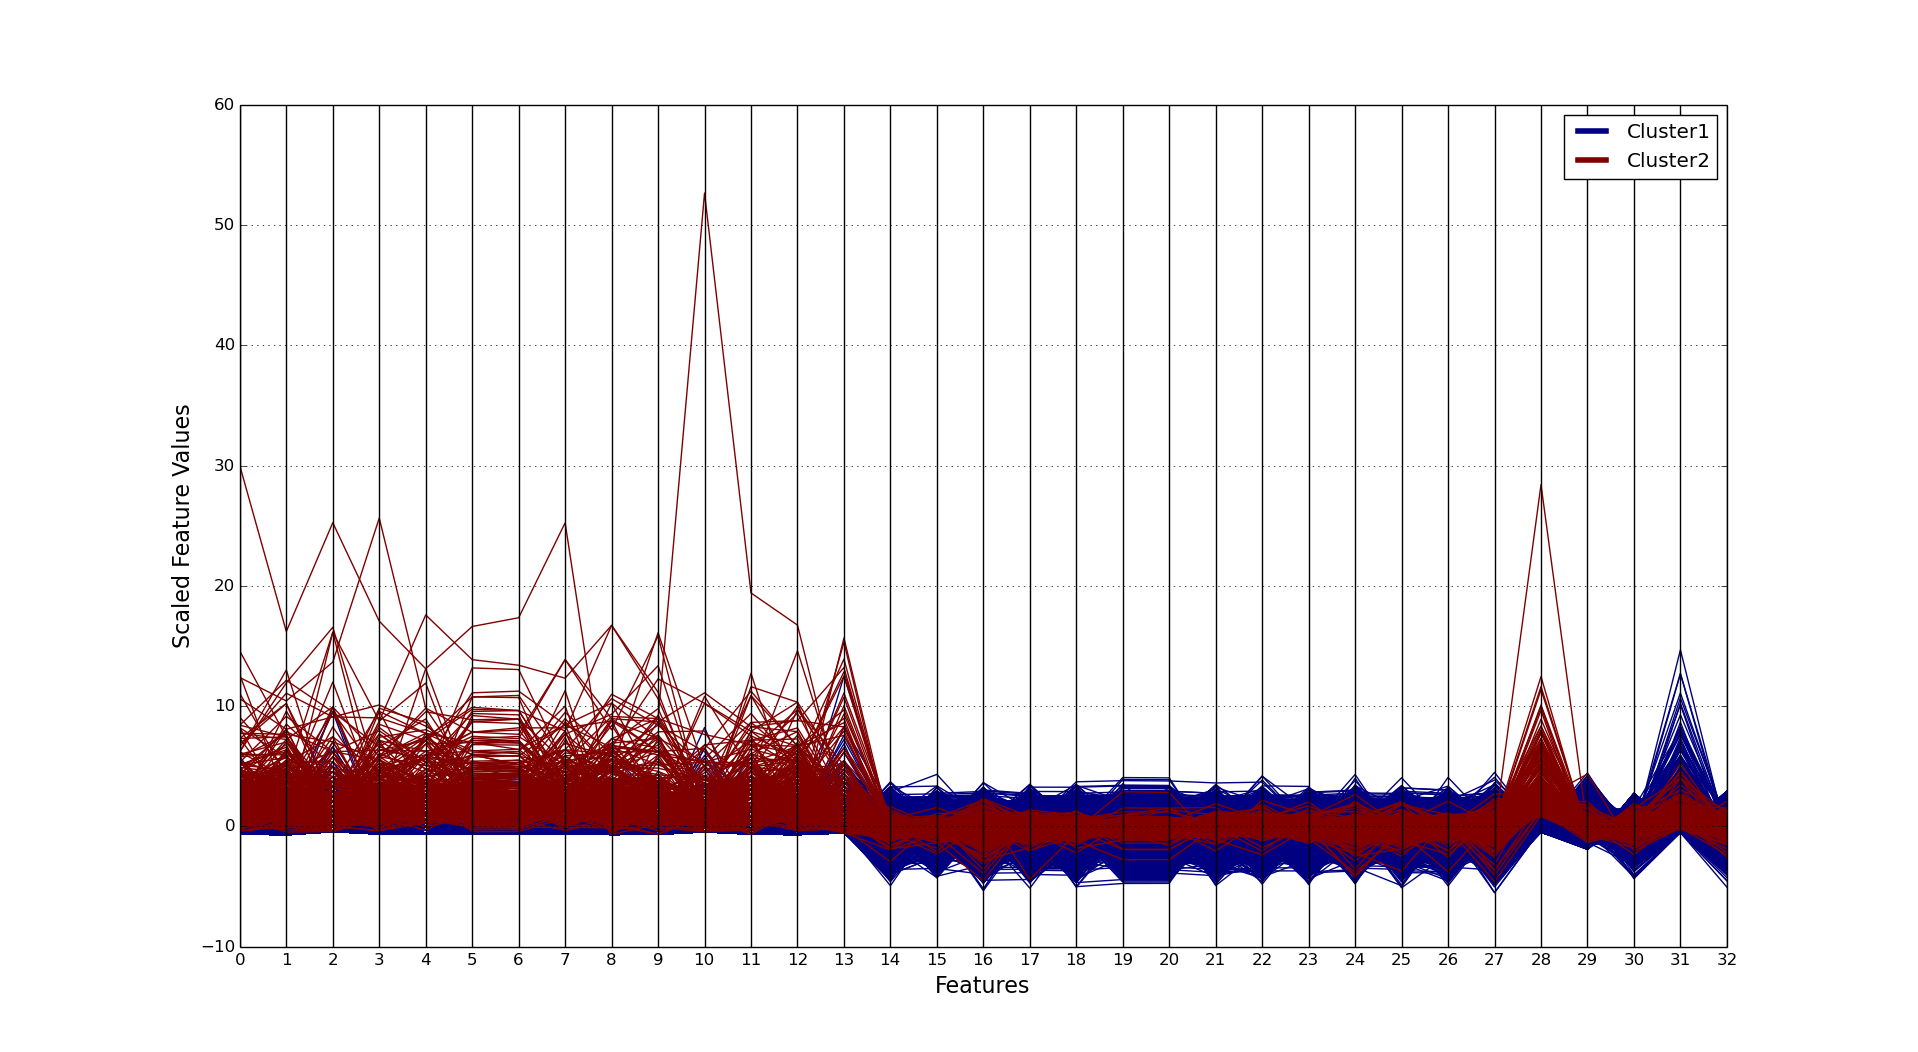
\includegraphics[width=0.9\textwidth]{old_features.png}
 	\caption{Plot of user features against the feature number for two clusters. Frequency features represent the total number of reviews a user gives a category. The feature vector for a given user forms a continuous line color coded by cluster. Feature values plotted on the $y$-axis are scaled by the mean and standard deviation.}
 	\label{fig:bad_clustering}
 \end{figure} 
 
 After applying this correction we observe clusters indicated in Figure \ref{fig:bad_clustering}. This shows that many features are influencing the choice of cluster boundaries, not just one. However, if we delve deeper into the results, we see that the dominant features are the frequency of which users attend restaurants of each category. In this first clustering attempt, the frequency features before scaling are simply the number of reviews a user has written for restaurants in each category. Notice that the clusters seem to be grouped by the number of users have written. This is not ideal since we would like to discriminate users based on preference, not the total number of reviews. The total number of reviews is a relevant feature and is captured in our feature set by the total number of reviews feature but we would prefer that it not dominate the cluster boundaries.
 
 To solve this issue, we re-engineer the category review frequency features. Instead of the features simply being the user's total number of reviews for each category, these features are normalized by the number of user reviews. Therefore, the bias of choosing clusters based on the number of reviews is reduced. The resulting clusters are shown in Figure \ref{fig:better_clustering} for 2 clusters. Notice that now the clusters are separating based on user preferences. For instance, users in cluster 1 tend to rate restaurants with nightlife or bars very poorly.

\begin{figure}[h!]
	\centering
	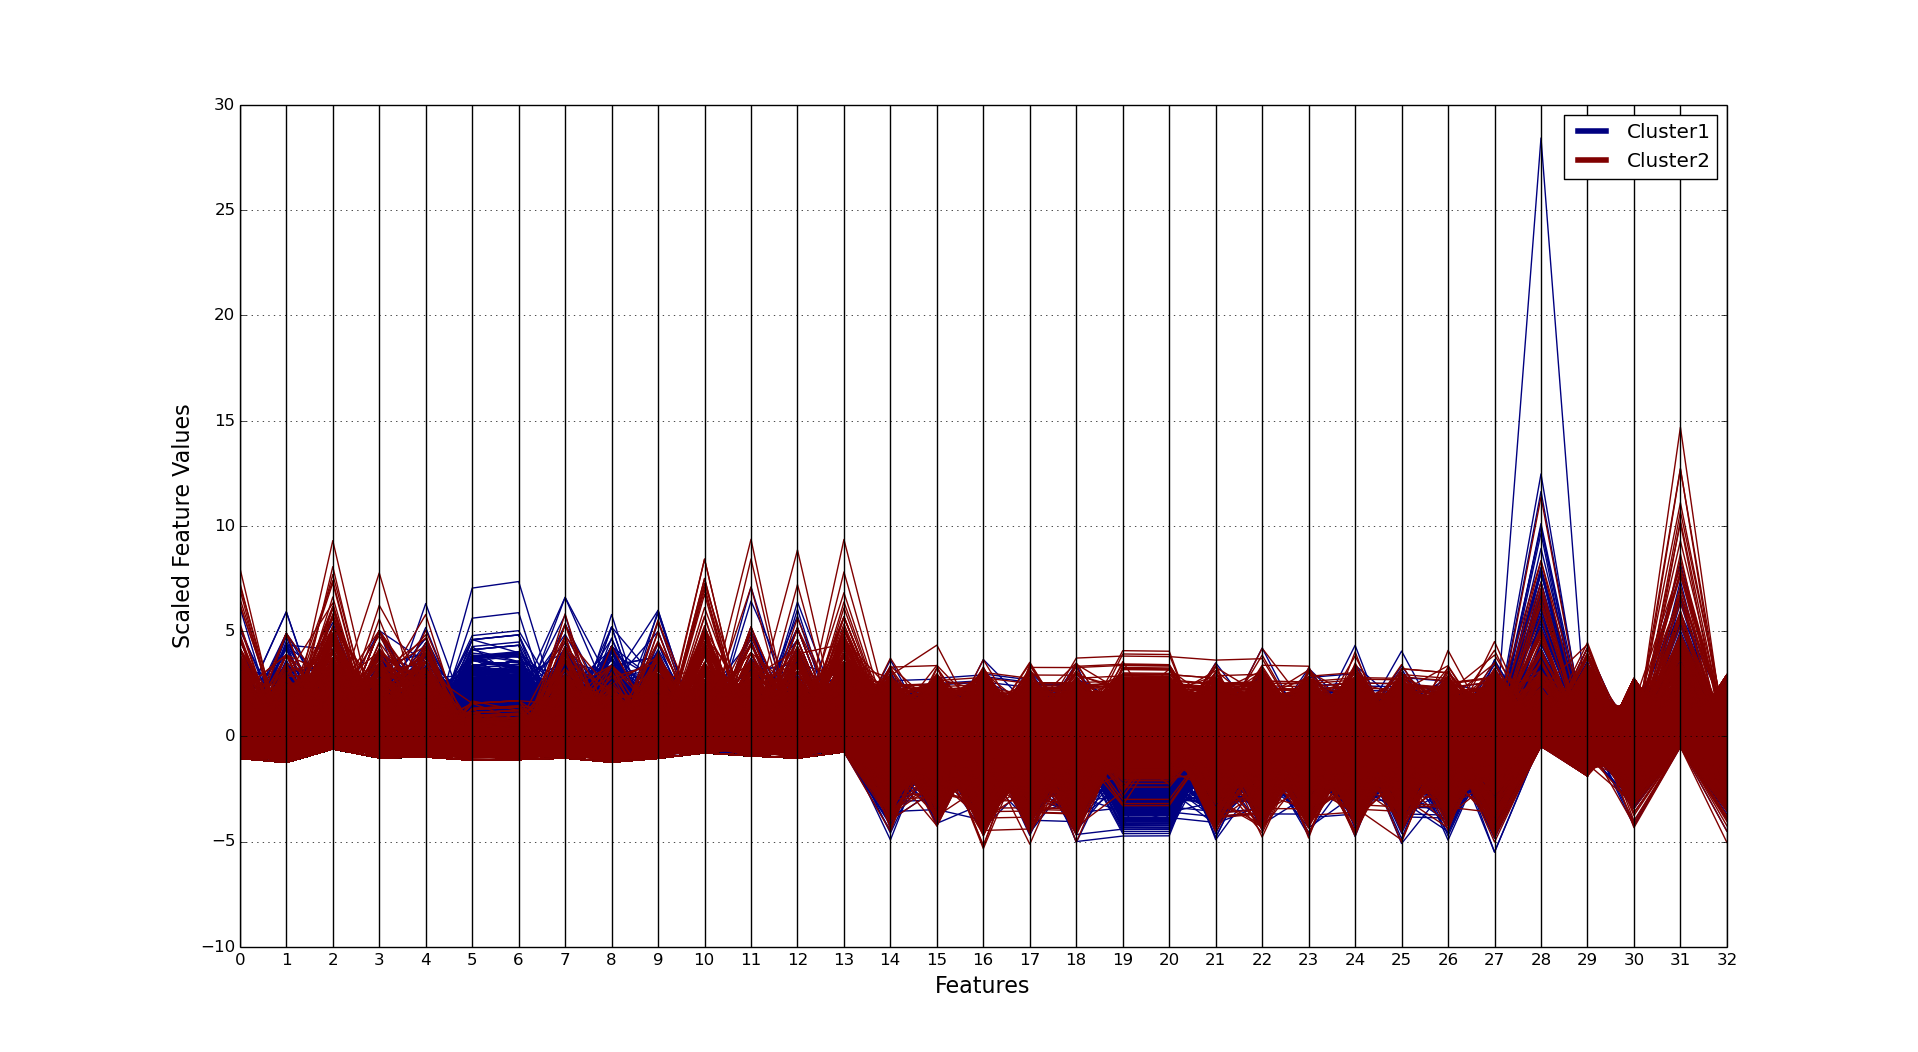
\includegraphics[width=0.9\textwidth]{kmeans2clusters_all.png}
	\caption{Plot of user features against the feature number for two clusters. Frequency features represent the fraction of a user's reviews that correspond to each category. The feature vector for a given user forms a continuous line color coded by cluster. Feature values plotted on the $y$-axis are scaled by the mean and standard deviation.}
	\label{fig:better_clustering}
\end{figure} 

When we extend to four clusters we see even more separation. This is shown in Figure~\ref{fig:kmeans_4}. Notice that now there is further separation based on preference. Clusters 1, 3, and 4 separate strongly based on ratings for restaurants with bars and nightlife. Cluster 2 strongly separates from the rest with a higher percentage of reviews on bars and restaurants.

\begin{figure}[h!]
	\centering
	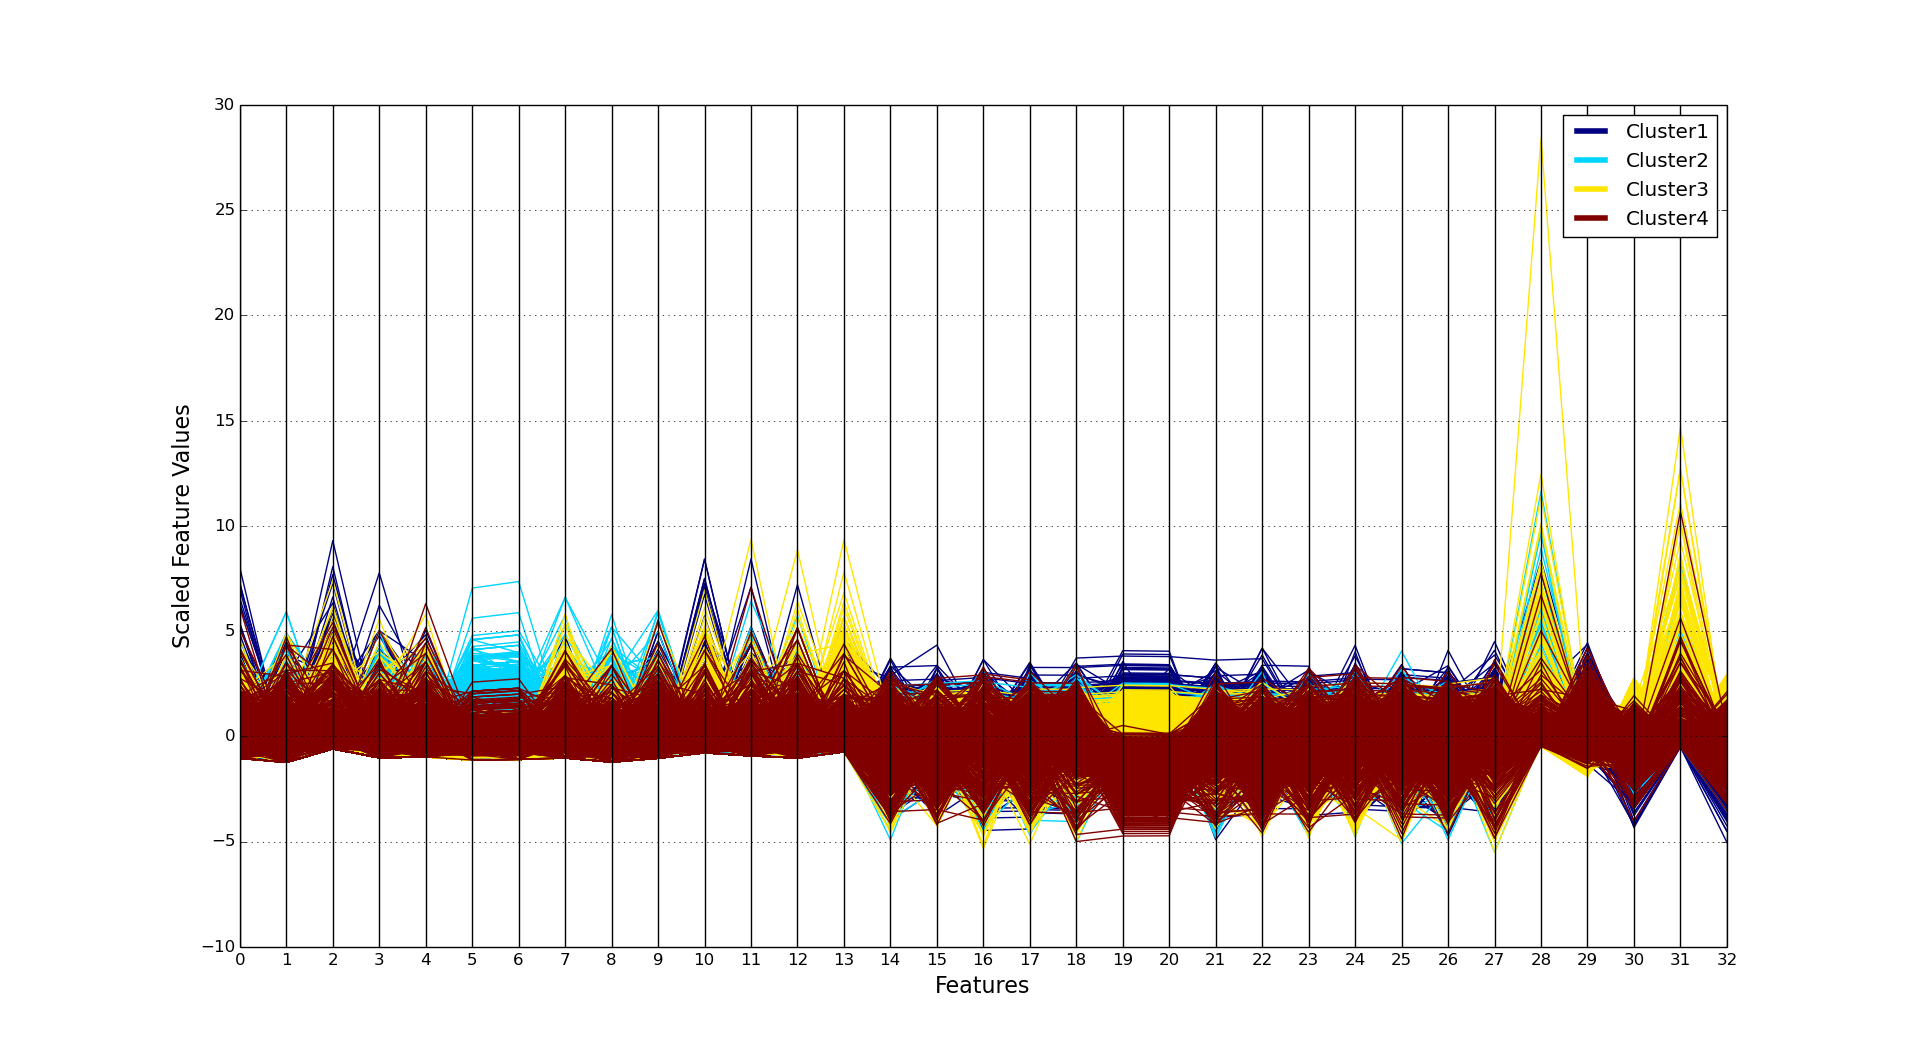
\includegraphics[width=0.9\textwidth]{kmeans4clusters_all.png}
	\caption{Plot of user features against the feature number for four restaurant clusters. The feature vector for a given user forms a continuous line color coded by cluster. Feature values plotted on the $y$-axis are scaled by the mean and standard deviation.}
	\label{fig:kmeans_4}
\end{figure}

While it is encouraging to see cluster separation, the large number of users can cause the data to be unreadable. Therefore, the average feature values for each cluster might be informative. These average values are presented for the case of four K-Means clusters in Figure~\ref{fig:kmeans_4_avg}. It is important to note that the cluster numbering is arbitrary and does not align with the cluster numbering shown in Figure~\ref{fig:kmeans_4}. 

\begin{figure}[h!]
	\centering
	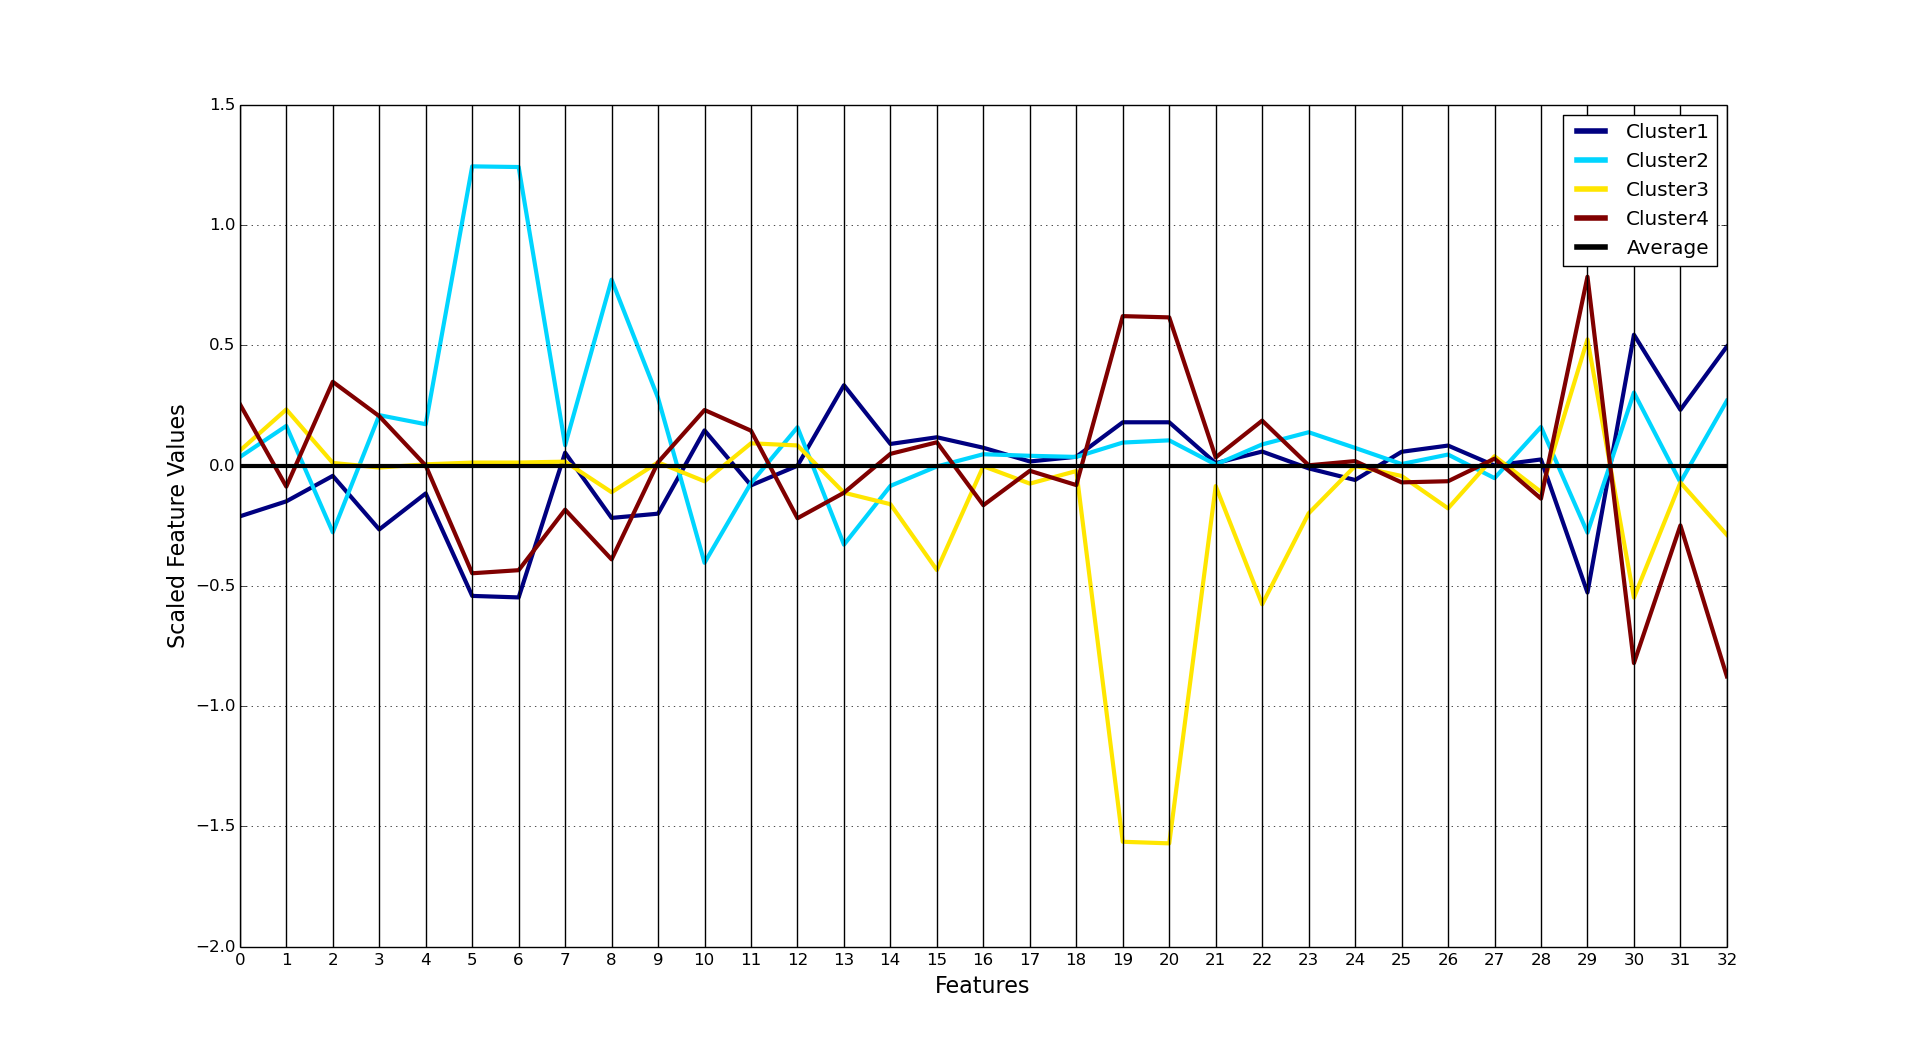
\includegraphics[width=0.9\textwidth]{kmeans4clusters.png}
	\caption{Cluster-averaged features plotted for every feature in four restaurant clusters. Feature values plotted on the $y$-axis are scaled by the mean and standard deviation.}
	\label{fig:kmeans_4_avg}
\end{figure}

We see similar trends as before with bars and nightlife being two categories that strongly separate the data. We can also see trends that are not as obvious form the previous plots. For instance, users who strongly dislike restaurants with bars and nightlife also strongly dislike American restaurants, both traditional and new. On the other hand, we notice that those who prefer restaurants with bars and nightlife rarely review breakfast restaurants and dislike fast food.

All of this analysis assumes that the distance metric used in the K-Means algorithm is accurately finding representative clusters. The merit of clustering will be able to be tested later when we predict a user's final rating. If this model has merit, then we should see an improvement over analogous models with no clustering.

\subsubsection{Nightlife}
Due to the strong division of users by nightlife preference in restaurants, we are encouraged to apply our same strategy to predicting a user's rating for businesses in the nightlife category. 

As we learned previously, results are much improved when the category review frequency attributes are chosen to be fractional values and the features are scaled properly. We see the same results for the nightlife prediction problem. For brevity, we skip to results for four clusters using the scaled and fractional features. The results are shown in Figure~\ref{fig:nl_kmeans_4} with cluster averages plotted in Figure~\ref{fig:nl_kmeans_4_avg}

\begin{figure}[h!]
	\centering
	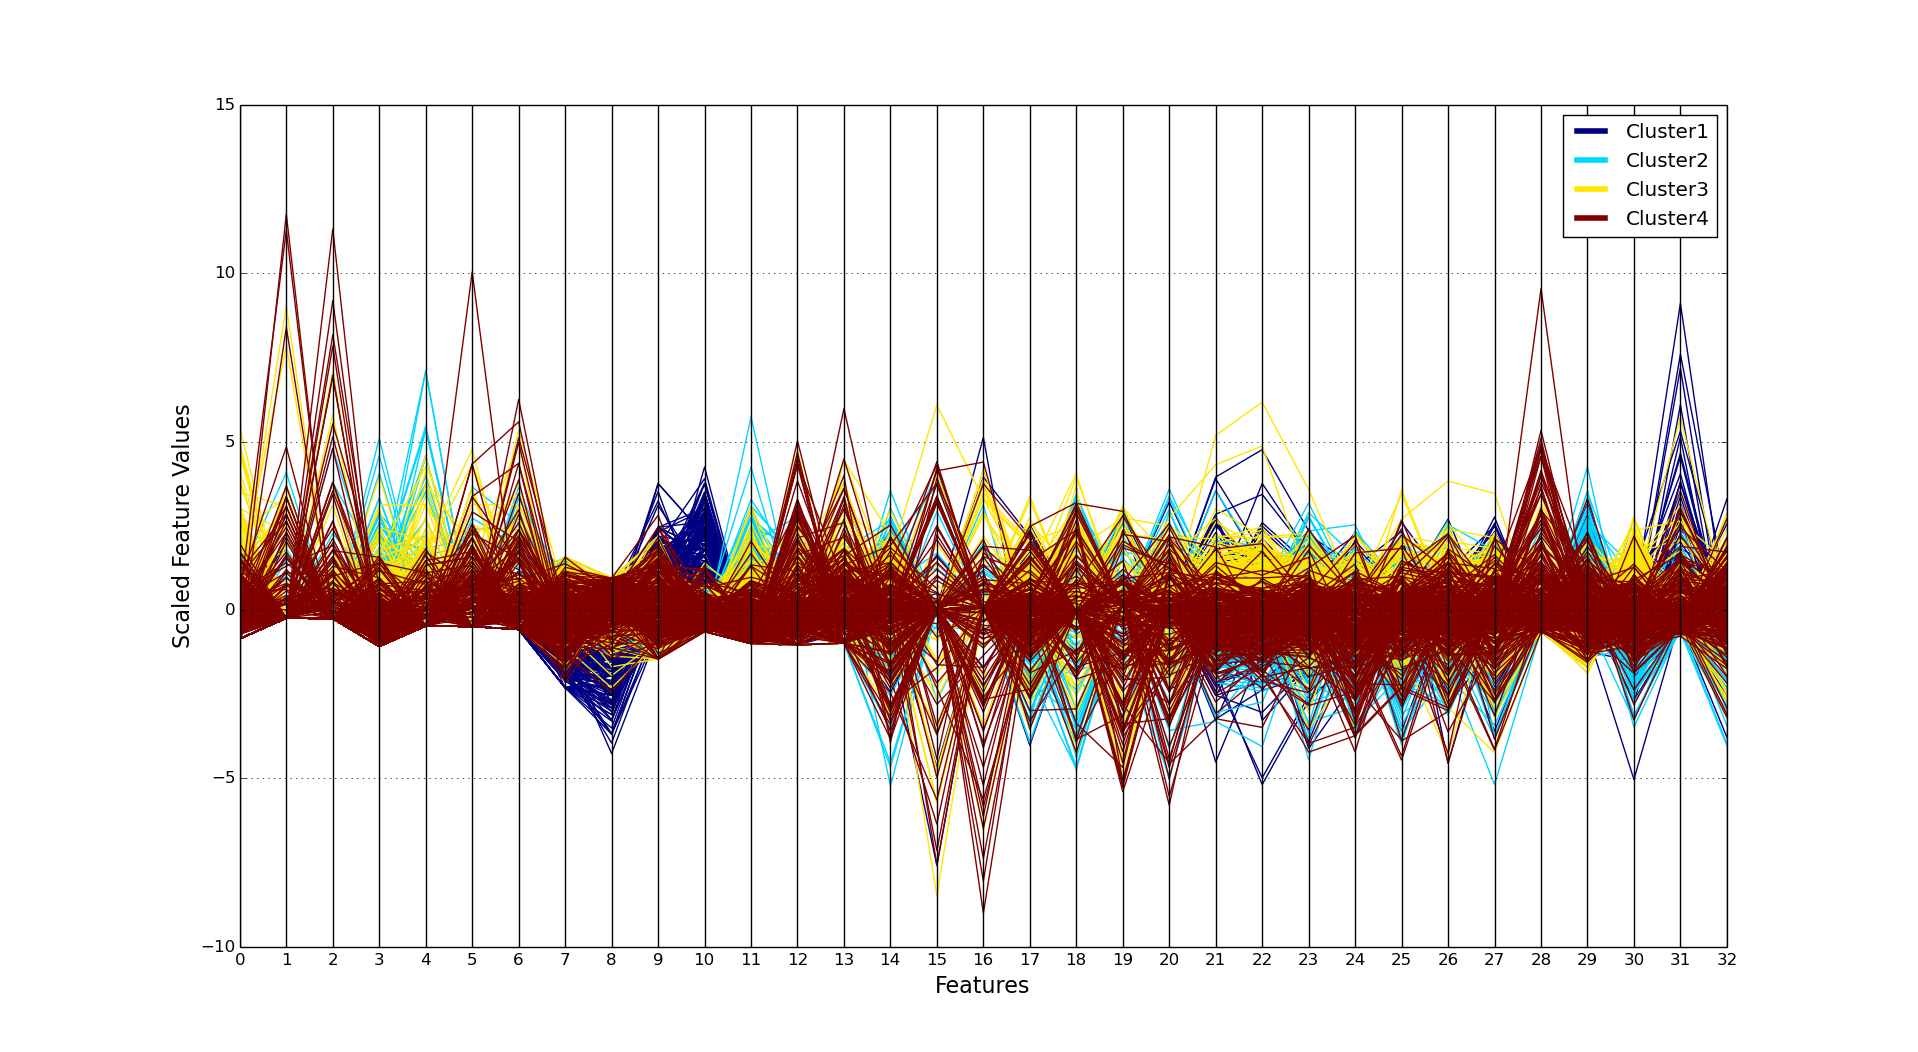
\includegraphics[width=0.9\textwidth]{NL_kmeans4clusters_all.png}
	\caption{Plot of user features against the feature number for four nightlife clusters. The feature vector for a given user forms a continuous line color coded by cluster. Feature values plotted on the $y$-axis are scaled by the mean and standard deviation.}
	\label{fig:nl_kmeans_4}
\end{figure}

\begin{figure}[h!]
	\centering
	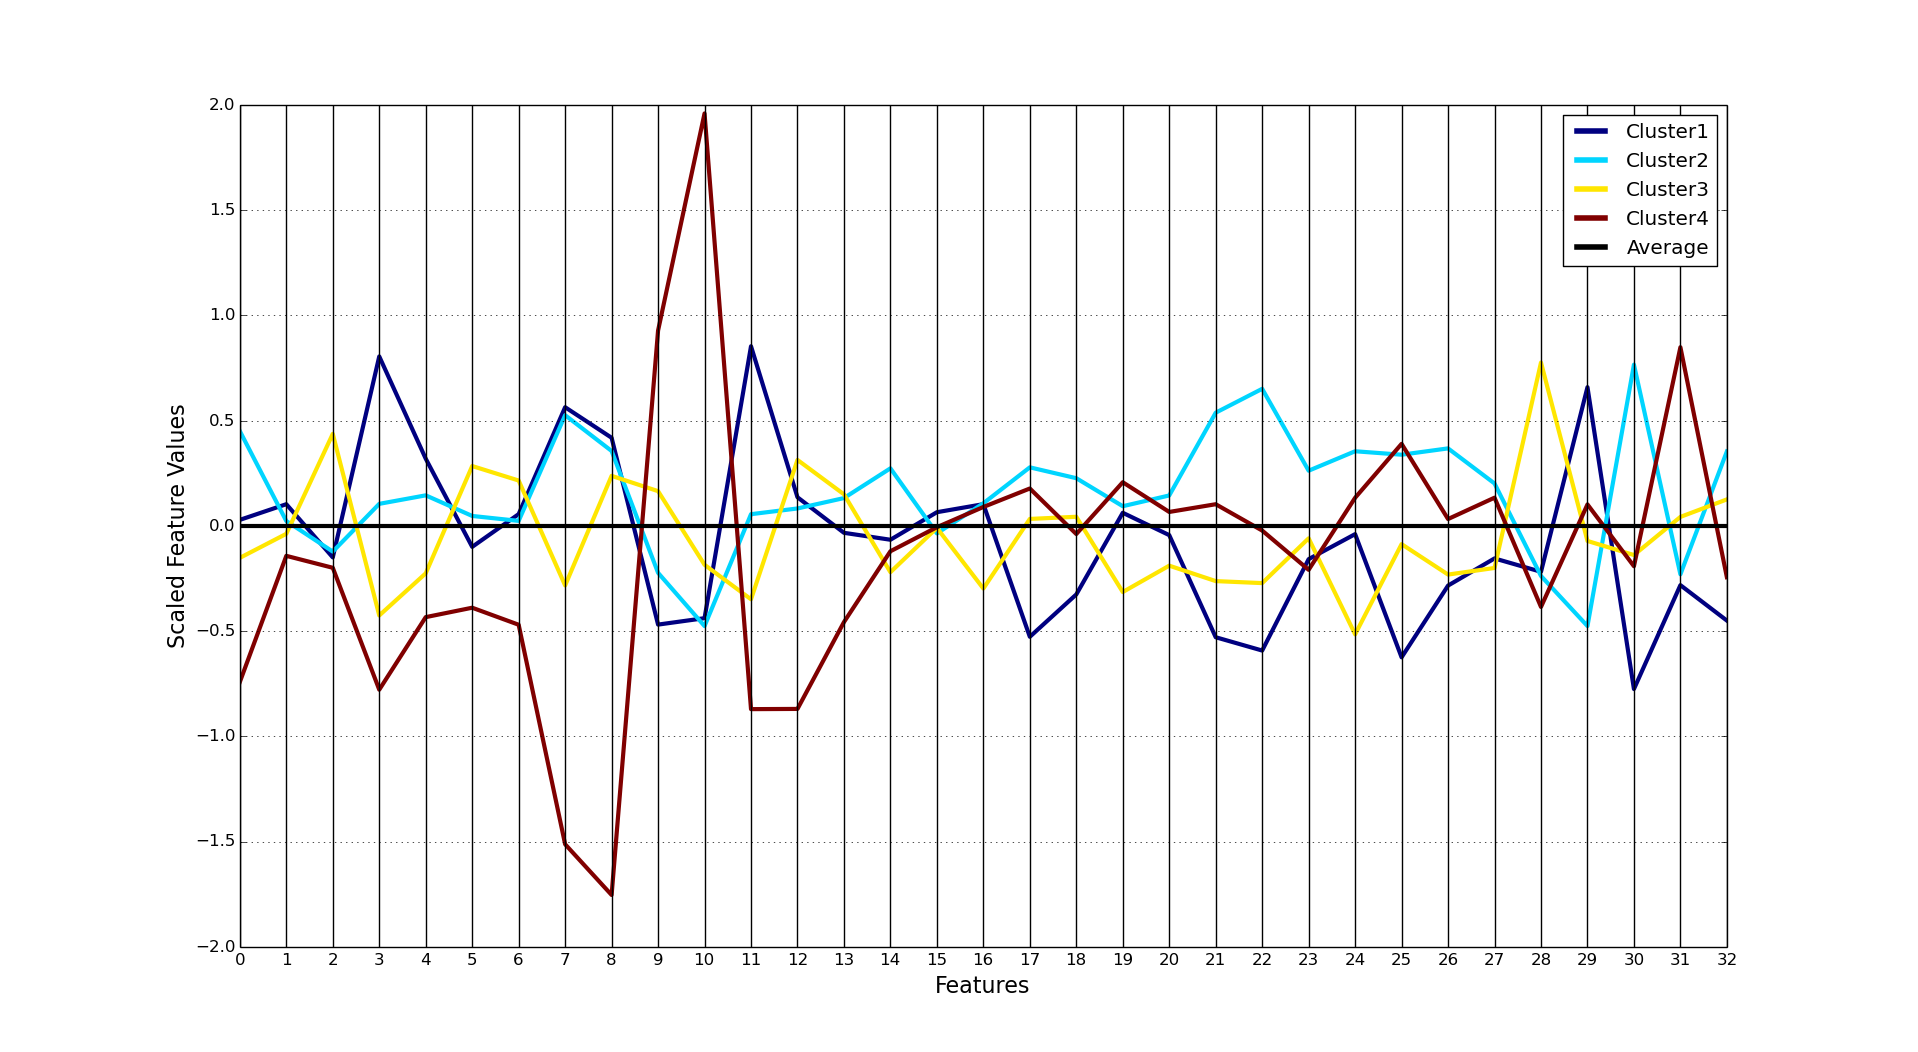
\includegraphics[width=0.9\textwidth]{NL_kmeans4clusters.png}
	\caption{Cluster-averaged features plotted for every feature in four nightlife clusters. Feature values plotted on the $y$-axis are scaled by the mean and standard deviation.}
	\label{fig:nl_kmeans_4_avg}
\end{figure}

These clusters show users that have a high number of dance club reviews do not often review bars, sports bars, or pubs. This same group often reviews lounges as well and tends to rate sports bars, karaoke, and music venues highly. Another cluster tends to review wine bars but not dance clubs. This group rates bars and lounges highly but rates jazz clubs poorly. Again, all of this analysis assumes that the clustering algorithm is functioning properly and finding real clusters in the data. We now will see how the clustering scheme affects the prediction of user ratings.

\subsubsection{Overall Trends}
For the overal system, we first chose a method of clustering (K-Means, K-Neighbors, or Gaussian Mixture), and a method for inference (MLE, lasso, ridge, or bayesian ridge). We then tested the system end-to-end with the partitions of the user and business data. We let the MLE inference method be the base line with which we compared all other regression methods, because it represents the most simple estimation. We report error in terms of the average absolute value difference between the guess and the actual rating. This error number must range from $[0, 5]$, where a lower number indicates we are making better guesses. Figure~\ref{fig:MLE} visually shows the result of varying the hyperparameter for K-Means, K-Neighbors, and Gaussian Mixtures.

\begin{figure}[h!]
    \begin{subfigure}[h!]{0.33\textwidth}
        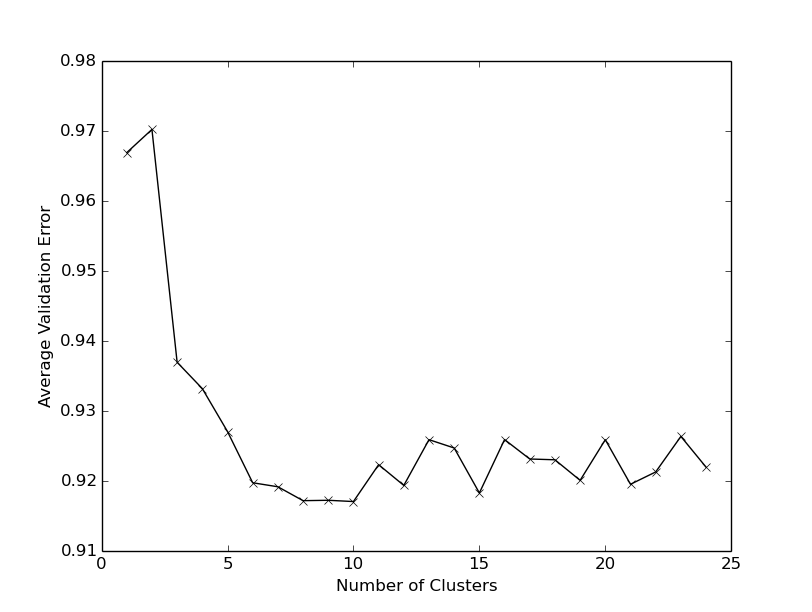
\includegraphics[width=\textwidth]{kmeans_mle.png}
        \caption{K-Means/MLE}
        \label{fig:kmMLE}
    \end{subfigure}%
    \begin{subfigure}[h!]{0.33\textwidth}
        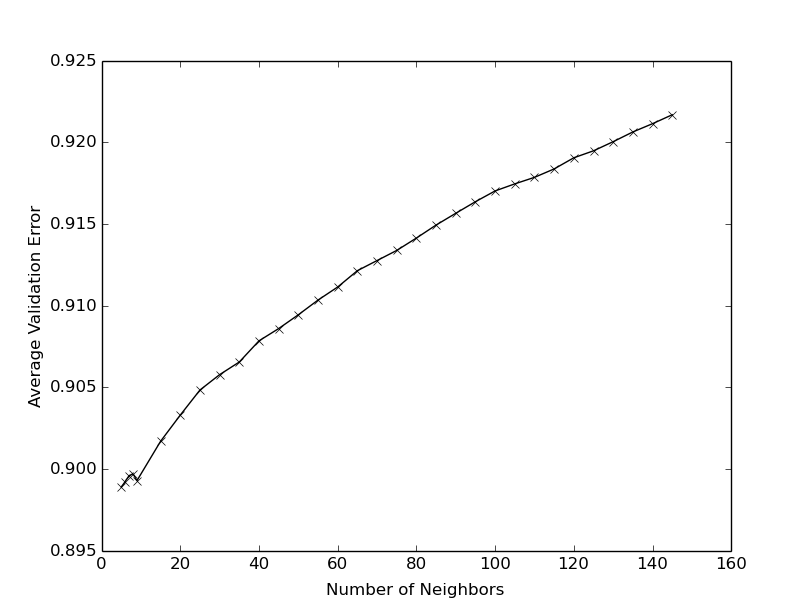
\includegraphics[width=\textwidth]{KN_mle.png}
        \caption{K-Neighbors/MLE}
        \label{fig:knMLE}
    \end{subfigure}
    \begin{subfigure}[h!]{0.33\textwidth}
        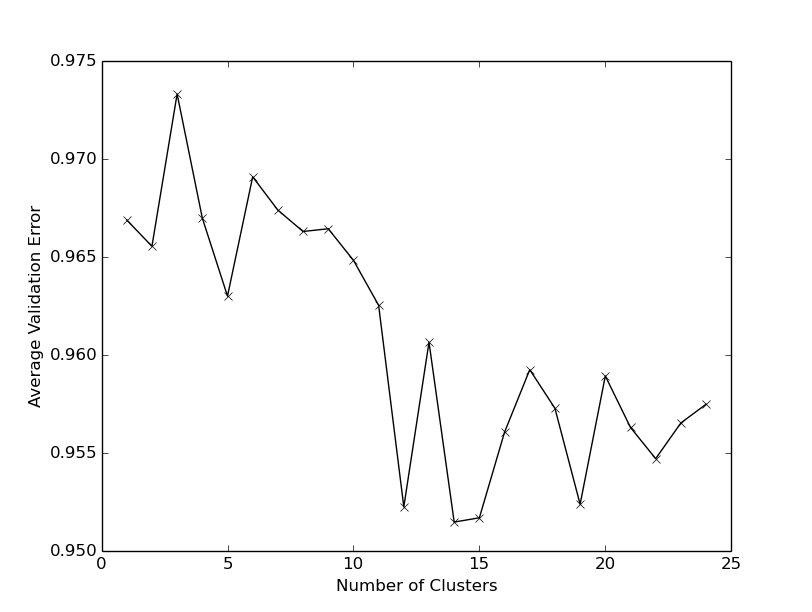
\includegraphics[width=\textwidth]{GM_mle.png}
        \caption{Gaussian Mixture/MLE}
        \label{fig:gmMLE}
    \end{subfigure}
    \caption{Running the three types of clustering using the MLE estimate for each individual inference problem. The x-axis represents the hyperparameter of the model (number of clusters, or number per cluster), and the y-parameter shows the error per review.}
    \label{fig:MLE}
\end{figure}

Note that K-Means selects the optimal number of clusters to be 8, while Gaussian Mixtures selects 14. The starting downwards trends in Figure~\ref{fig:kmMLE} and Figure~\ref{fig:gmMLE} shows that custering is having an effect on the error rate. If adding more clusters is resulting in a lower error, it is evidence that the clusters are finding categories of similar users, and that these cateories are successfully differentiating between different users' tastes.

We find that the K-Neighbors approach is not working as well as the other two. An explanation of this is that the k nearest-neighbors to a single point may not necessarily be users with similar tastes, because we have many dimensions in the user feature vector. Another explanation is that the users belong distinctly in different categories, and forcing the method to use the k nearest-neighbors instead of the category is forcing a mixture of users who have varying tastes. This provides further evidence of the existence of user similarity groups. Table~\ref{tab:baseline} shows the numerical results from running the test set with the hyperparameter that returned the lowest error for the validation set.

\begin{table}[h!]
    \begin{tabularx}{0.9\textwidth}{| X | r | r | r | }
        \hline
        Method & Hyperparameter & Validation Error & Test Error \\
        \hline
        K-Means & 8 & 0.917 & 0.912 \\
        K-Neighbors & 1 & 0.899 & 0.954 \\
        Gaussian Mixture & 14 & 0.951 & 0.943\\
        \hline
    \end{tabularx}
    \caption{The lowest validation error achieved and the corresponding test error for K-Means, K-Neighbors, and Gaussian Mixtures for the hidden variable, and MLE for the inference model per cluster. This is our baseline to which we will compare the other methods.}
    \label{tab:baseline}
\end{table}

Next, we compare the different types of inference methods to MLE. For each hidden variable method (K-Means, K-Neighbors, Gaussian Mixtures), we run the testing scheme using lasso, ridge, and bayesian ridge as our models of regression. We pick the model that achieves the lowest error on the end-to-end validation set. Figure~\ref{fig:BEST} shows optimal method chosen by each hidden variable method, and the effect of varying its hyperparameter for that method. 

\begin{figure}[h!]
    \begin{subfigure}[h!]{0.33\textwidth}
        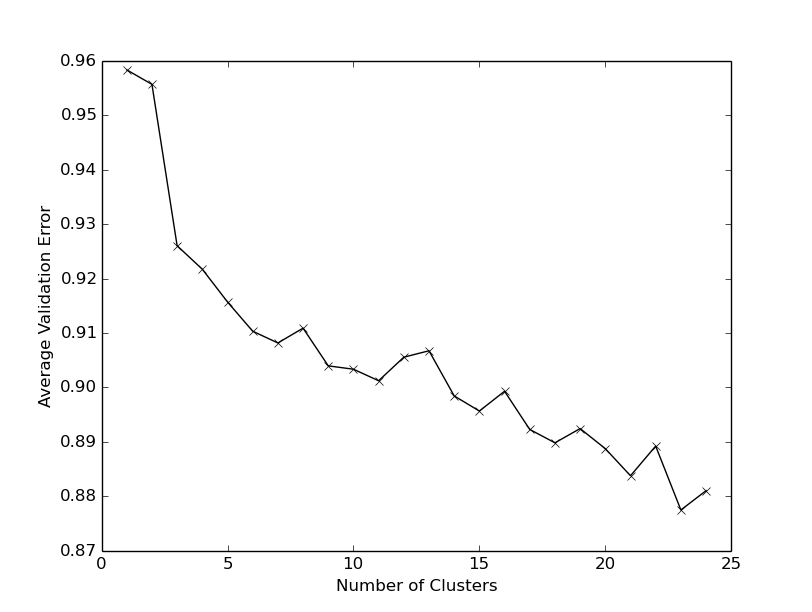
\includegraphics[width=\textwidth]{kmeans_lasso.png}
        \caption{K-Means/Lasso}
        \label{fig:kmBEST}
    \end{subfigure}%
    \begin{subfigure}[h!]{0.33\textwidth}
        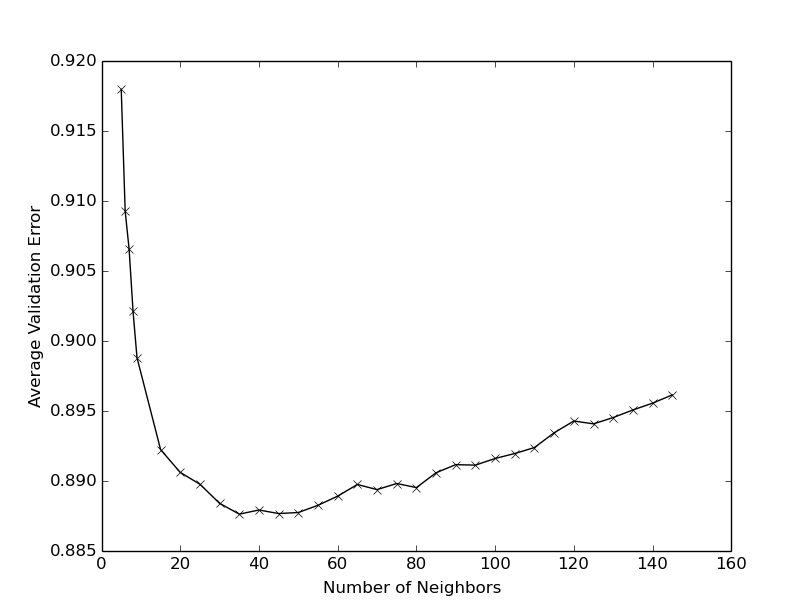
\includegraphics[width=\textwidth]{KN_ridge.png}
        \caption{K-Neighbors/Ridge}
        \label{fig:knBEST}
    \end{subfigure}
    \begin{subfigure}[h!]{0.33\textwidth}
        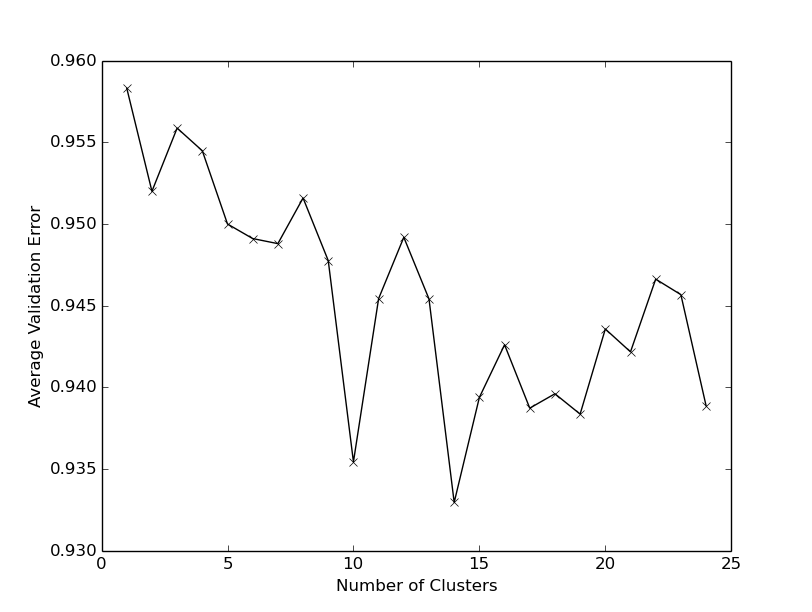
\includegraphics[width=\textwidth]{GM_lasso.png}
        \caption{Gaussian Mixture/Lasso}
        \label{fig:gmBEST}
    \end{subfigure}
    \caption{Running the three types of clustering on the best model of inference for each, as determined by the validation error.}
    \label{fig:BEST}
\end{figure}

We are also interested to see how the error changed between using MLE as the inference model, versus using an actual regression model. Overall, we find that all the regression models show a lower error rate than using the MLE, which provides evidence that the second non-hidden variable also works to improve the accuracy. Table~\ref{tab:improvement} shows results from this portion.

\begin{table}[h!]
    \begin{tabularx}{0.9\textwidth}{| r | X | r | X | X | X |}
        \hline
        Cluster Method & Model Method & Hyperparam & Validation Error & Test Error & \% Improvement\\
        \hline
        K-Means & Lasso & 24 & 0.877 & 0.861 & 5.59 \\
        K-Neighbors & Ridge & 39 & 0.886 & 0.907 & 4.93 \\
        Gaussian Mixture & Lasso & 14 & 0.932 & 0.938 & 0.53 \\
        \hline
    \end{tabularx}
    \caption{The lowest validation error achieved and the corresponding test error for K-Means, K-Neighbors, and Gaussian Mixtures for the hidden variable, for different types of inference models. The improvement is measured relative to the test error for the MLE case.}
    \label{tab:improvement}
\end{table}

For Gaussian Mixtures, there seems to be minimal improvement as comared to the MLE method. However, both K-Means and K-Neighbors enjoy a 5\% improvement when using a regression method for the second variable instead of the maximum liklihood estimate.

Overall, we have evidence that both variables contribute to improving the predicted error rate. For the hidden variable, the evidence comes from the fact that adding more clusters seems drives down the error. This means that the clusters are contributing to a correct prediction by grouping similar users together. For the non-hidden variable, this evidence comes from the fact that using a regression model for inference shows an improvement in error over using the MLE.

\subsubsection{Overall Trends in Nightlife}
For the nightlife category, we apply the same techniques as the overall restaurant category. First, we compare the different methods using the MLE estimate for inference of the second variable. The effect of varying the hyperparameter for each is shown in Figure~\ref{fig:MLE_NL}.

\begin{figure}[h!]
    \begin{subfigure}[h!]{0.33\textwidth}
        \includegraphics[width=\textwidth]{NL_kmeans_mle.png}
        \caption{K-Means/MLE}
        \label{fig:kmMLE_NL}
    \end{subfigure}%
    \begin{subfigure}[h!]{0.33\textwidth}
        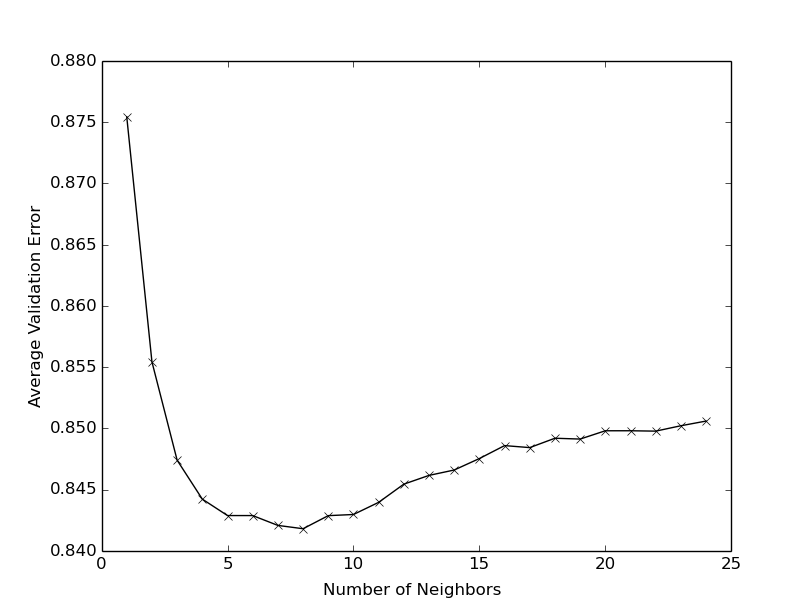
\includegraphics[width=\textwidth]{NL_KN_mle.png}
        \caption{K-Neighbors/MLE}
        \label{fig:knMLE_NL}
    \end{subfigure}
    \begin{subfigure}[h!]{0.33\textwidth}
        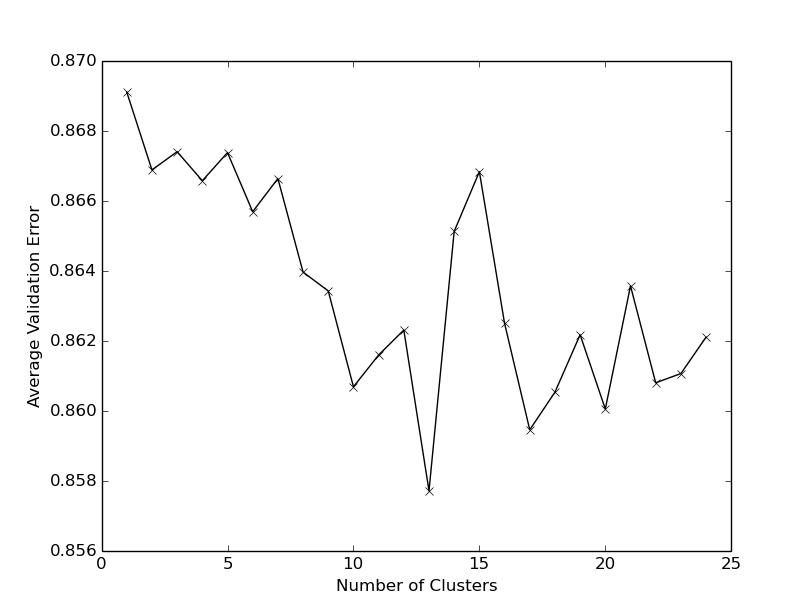
\includegraphics[width=\textwidth]{NL_GM_mle.png}
        \caption{Gaussian Mixture/MLE}
        \label{fig:gmMLE_NL}
    \end{subfigure}
    \caption{Running the three types of clustering using the MLE estimate for each individual inference problem, only with restaurants in the nightlife category.}
    \label{fig:MLE_NL}
\end{figure}

We find that the results here show generally the same trends as the previous results, except the K-Neighbors model, which seems to be performing optimally at 8 clusters. We notice here that at the beginning of the graph in Figure~\ref{fig:knMLE_NL}, the error rate goes down with the number of users in a cluster. Unlike the previous section, where we used all categories of restaurants, looking at k nearest-neighbors seems to be helping make a better prediction. This may because because, based on the data, individuals tend to have strong preferences about bars. This can mean that the groups of similar users are spread out from other groups in feature space, but densely populated within themselves. This means that looking at the k-nearest neighbors essentially looks at users in the same cluster as the queried user, leading to better results.

Overall, the error rate in the night life category is lower than that of the previous section, as shown in Table~\ref{tab:baseline_NL}. This is not suprising if we assume that users have strong preferences about nightlife.

\begin{table}[h!]
    \begin{tabularx}{0.9\textwidth}{| X | r | r | r | r |}
        \hline
        Method & Hyperparam & Validation Error & Test Error & \% Change\\
        \hline
        K-Means &  20 & 0.836 & 0.843 & 7.43 \\
        K-Neighbors &  8 & 0.842 & 0.846 & 11.32 \\
        Gaussian Mixture & 13 & 0.857 & 0.861 & 8.70 \\
        \hline
    \end{tabularx}
    \caption{The lowest validation error achieved and the corresponding test error for K-Means, K-Neighbors, and Gaussian Mixtures for the hidden variable, and MLE for the inference model per cluster, only within the nighlife category. The \% Change is the improvement as compared to the test data in Table~\ref{tab:baseline}, MLE estimates for all restaurant data.}
    \label{tab:baseline_NL}
\end{table}

Finally, we also try using regression models for the second variable. We show the results of varying the hyperparameter for the regression model that yields the lowest error, for each K-Mean, K-Neighbors, and Gaussian Mixtures in Figure~\ref{fig:BEST_NL}.

\begin{figure}[h!]
    \begin{subfigure}[h!]{0.33\textwidth}
        \includegraphics[width=\textwidth]{NL_kmeans_ridge.png}
        \caption{K-Means/Ridge}
        \label{fig:kmBEST}
    \end{subfigure}%
    \begin{subfigure}[h!]{0.33\textwidth}
        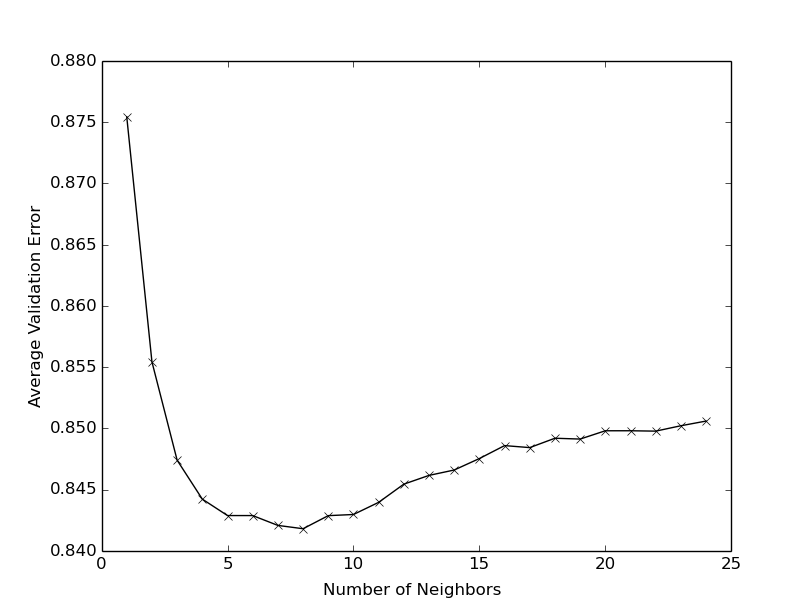
\includegraphics[width=\textwidth]{NL_KN_mle.png}
        \caption{K-Neighbors/MLE}
        \label{fig:knBEST}
    \end{subfigure}
    \begin{subfigure}[h!]{0.33\textwidth}
        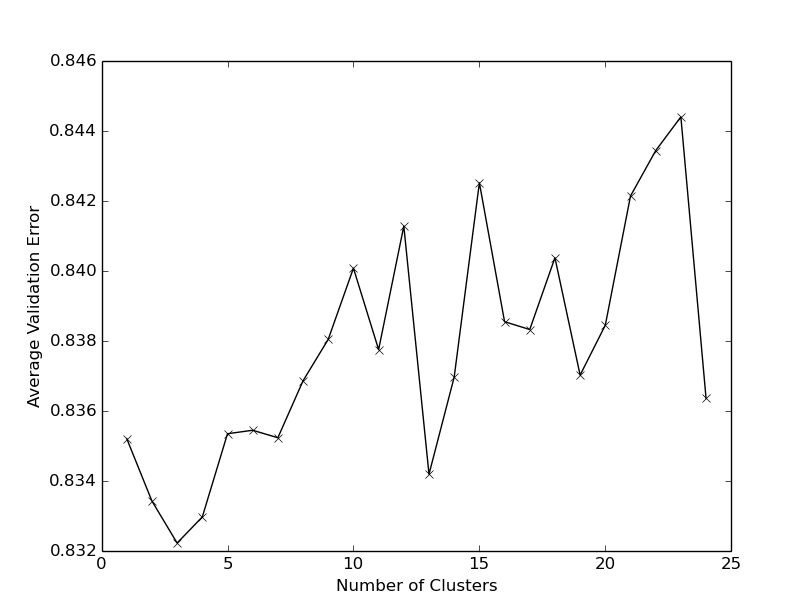
\includegraphics[width=\textwidth]{NL_GM_ridge.png}
        \caption{Gaussian Mixture/Ridge}
        \label{fig:gmBEST}
    \end{subfigure}
    \caption{Running the three types of clustering on the best model of inference for each, as determined by the validation error, for only the nighlife category.}
    \label{fig:BEST_NL}
\end{figure}

As before, we can also look at the test error rates for each of these systems. These are reported in Table~\ref{tab:improvement_NL}, where Improvement is shown relative to the MLE results.

\begin{table}[h!]
    \begin{tabularx}{0.9\textwidth}{| r | X | r | X | X | X |}
        \hline
        Cluster Method & Model Method & Hyperparam & Validation Error & Test Error & \% Improvement\\
        \hline
        K-Means & Ridge & 4 & 0.780 & 0.801 & 4.98 \\
        K-Neighbors & MLE & 8 & 0.842 & 0.846 & 0.00 \\
        Gaussian Mixture & Ridge & 3 & 0.832 & 0.831 & 3.60 \\
        \hline
    \end{tabularx}
    \caption{The lowest validation error achieved and the corresponding test error for K-Means, K-Neighbors, and Gaussian Mixtures for the hidden variable, and different inference type of inference models, only with nightlife. The \% Improvement is the improvement upon the test results in Table~\ref{tab:baseline_NL}.}
    \label{tab:improvement_NL}
\end{table}

Note that the K-Neighbors seems to favor MLE in this case over all the other tested regression models. In constrast, K-Means and Gaussian Mixture both favor using ridge regression for the individual models. We can also see that substituting the ridge regression instead of the MLE in these two cases does not affect the error rate as significantly as it did in the previous section. This confirms are belief that users have strong preferences with nightlife, as the clusters themselves figure out the preferences and there is not much more room for the regression to figure out a trend when compared to the maximum liklihood estimate.

Overall we see that the hidden variable is most important when users have strong preferences and can fall easily within groups. If the preferences are moderate, the groups are close together, and it's likely that the second variable's regressio method will also lower the error rate.
% \subsection{Regression}
% \subsubsection{Maximum Liklihood Estimate}
% \subsubsection{Bayesian Ridge}
% \subsubsection{Lasso}
% \subsubsection{Random Forest}

\section{References}

\end{document}
